% Options for packages loaded elsewhere
\PassOptionsToPackage{unicode}{hyperref}
\PassOptionsToPackage{hyphens}{url}
\PassOptionsToPackage{dvipsnames,svgnames,x11names}{xcolor}
%
\documentclass[
  ignorenonframetext,
]{beamer}
\usepackage{pgfpages}
\setbeamertemplate{caption}[numbered]
\setbeamertemplate{caption label separator}{: }
\setbeamercolor{caption name}{fg=normal text.fg}
\beamertemplatenavigationsymbolsempty
% Prevent slide breaks in the middle of a paragraph
\widowpenalties 1 10000
\raggedbottom
\setbeamertemplate{part page}{
  \centering
  \begin{beamercolorbox}[sep=16pt,center]{part title}
    \usebeamerfont{part title}\insertpart\par
  \end{beamercolorbox}
}
\setbeamertemplate{section page}{
  \centering
  \begin{beamercolorbox}[sep=12pt,center]{part title}
    \usebeamerfont{section title}\insertsection\par
  \end{beamercolorbox}
}
\setbeamertemplate{subsection page}{
  \centering
  \begin{beamercolorbox}[sep=8pt,center]{part title}
    \usebeamerfont{subsection title}\insertsubsection\par
  \end{beamercolorbox}
}
\AtBeginPart{
  \frame{\partpage}
}
\AtBeginSection{
  \ifbibliography
  \else
    \frame{\sectionpage}
  \fi
}
\AtBeginSubsection{
  \frame{\subsectionpage}
}
\usepackage{amsmath,amssymb}
\usepackage{lmodern}
\usepackage{iftex}
\ifPDFTeX
  \usepackage[T1]{fontenc}
  \usepackage[utf8]{inputenc}
  \usepackage{textcomp} % provide euro and other symbols
\else % if luatex or xetex
  \usepackage{unicode-math}
  \defaultfontfeatures{Scale=MatchLowercase}
  \defaultfontfeatures[\rmfamily]{Ligatures=TeX,Scale=1}
\fi
% Use upquote if available, for straight quotes in verbatim environments
\IfFileExists{upquote.sty}{\usepackage{upquote}}{}
\IfFileExists{microtype.sty}{% use microtype if available
  \usepackage[]{microtype}
  \UseMicrotypeSet[protrusion]{basicmath} % disable protrusion for tt fonts
}{}
\makeatletter
\@ifundefined{KOMAClassName}{% if non-KOMA class
  \IfFileExists{parskip.sty}{%
    \usepackage{parskip}
  }{% else
    \setlength{\parindent}{0pt}
    \setlength{\parskip}{6pt plus 2pt minus 1pt}}
}{% if KOMA class
  \KOMAoptions{parskip=half}}
\makeatother
\usepackage{xcolor}
\newif\ifbibliography
\usepackage{graphicx}
\makeatletter
\def\maxwidth{\ifdim\Gin@nat@width>\linewidth\linewidth\else\Gin@nat@width\fi}
\def\maxheight{\ifdim\Gin@nat@height>\textheight\textheight\else\Gin@nat@height\fi}
\makeatother
% Scale images if necessary, so that they will not overflow the page
% margins by default, and it is still possible to overwrite the defaults
% using explicit options in \includegraphics[width, height, ...]{}
\setkeys{Gin}{width=\maxwidth,height=\maxheight,keepaspectratio}
% Set default figure placement to htbp
\makeatletter
\def\fps@figure{htbp}
\makeatother
\setlength{\emergencystretch}{3em} % prevent overfull lines
\providecommand{\tightlist}{%
  \setlength{\itemsep}{0pt}\setlength{\parskip}{0pt}}
\setcounter{secnumdepth}{-\maxdimen} % remove section numbering
\usepackage{graphicx}
\usepackage{bm}
\usepackage{array}
\usepackage{amsmath}
\usepackage{amsthm}
\usepackage{amsfonts}
\usepackage{amssymb}
\usepackage{tikz-cd}
\usepackage{url}
\definecolor{foreground}{RGB}{255,255,255}
\definecolor{background}{RGB}{34,28,54}
\definecolor{title}{RGB}{105,165,255}
\definecolor{gray}{RGB}{175,175,175}
\definecolor{lightgray}{RGB}{225,225,225}
\definecolor{subtitle}{RGB}{232,234,255}
\definecolor{hilight}{RGB}{112,224,255}
\definecolor{vhilight}{RGB}{255,111,207}
\setbeamertemplate{footline}[page number]
\ifLuaTeX
  \usepackage{selnolig}  % disable illegal ligatures
\fi
\IfFileExists{bookmark.sty}{\usepackage{bookmark}}{\usepackage{hyperref}}
\IfFileExists{xurl.sty}{\usepackage{xurl}}{} % add URL line breaks if available
\urlstyle{same} % disable monospaced font for URLs
\hypersetup{
  pdftitle={STAT 528 - Advanced Regression Analysis II},
  pdfauthor={Exponential family theory (part 3)},
  colorlinks=true,
  linkcolor={Maroon},
  filecolor={Maroon},
  citecolor={Blue},
  urlcolor={blue},
  pdfcreator={LaTeX via pandoc}}

\title{STAT 528 - Advanced Regression Analysis II}
\author{Exponential family theory (part 3)}
\date{}
\institute{Daniel J. Eck\\
Department of Statistics\\
University of Illinois}

\begin{document}
\frame{\titlepage}

\begin{frame}
\newcommand{\R}{\mathbb{R}}
\newcommand{\Prob}{\mathbb{P}}
\newcommand{\Proj}{\textbf{P}}
\newcommand{\Hcal}{\mathcal{H}}
\newcommand{\rootn}{\sqrt{n}}
\newcommand{\p}{\mathbf{p}}
\newcommand{\E}{\text{E}}
\newcommand{\Var}{\text{Var}}
\newcommand{\Cov}{\text{Cov}}

\newtheorem{cor}{Corollary}
\newtheorem{lem}{Lemma}
\newtheorem{thm}{Theorem}
\newtheorem{defn}{Definition}
\newtheorem{prop}{Proposition}
\end{frame}

\begin{frame}{Last time}
\protect\hypertarget{last-time}{}
\begin{itemize}
\tightlist
\item
  mean value parameters
\item
  maximum likelihood estimation (MLE)
\item
  asymptotics of MLE
\item
  finite sample concentration of MLE
\end{itemize}
\end{frame}

\begin{frame}{Learning Objectives Today}
\protect\hypertarget{learning-objectives-today}{}
\begin{itemize}
\tightlist
\item
  generalized linear models (GLMs)
\item
  different parameterizations
\item
  motivation of logistic regression
\item
  inference
\end{itemize}
\end{frame}

\begin{frame}{Canonical linear submodels: intro to GLMs}
\protect\hypertarget{canonical-linear-submodels-intro-to-glms}{}
We now motivate generalized linear models (GLMs) within the context of
exponential theory.

A canonical affine submodel of an exponential family is a submodel
having parameterization \[
  \theta = a + M\beta
\] where:

\begin{itemize}
\tightlist
\item
  \(\theta \in \mathbb{R}^n\) is the canonical parameter vector
\item
  \(\beta \in \mathbb{R}^p\) is the canonical parameter vector for the
  submodel
\item
  \(a \in \mathbb{R}^n\) is a known offset vector
\item
  \(M \in \mathbb{R}^{n\times p}\) is a known \emph{model matrix}.
\end{itemize}
\end{frame}

\begin{frame}{}
\protect\hypertarget{section}{}
In most applications the offset vector is not used giving
parameterization \[
  \theta = M\beta,
\]\\
in which case we say the submodel is a \emph{canonical linear submodel}.

We will restrict attention to the canonical linear submodel in this
class.
\end{frame}

\begin{frame}{}
\protect\hypertarget{section-1}{}
The canonical linear submodel log likelihood is given by
\begin{equation} \label{subloglike}
\begin{split}
  l(\theta) &= \langle y,\theta\rangle - c(\theta) \\
    &= \langle y,M\beta\rangle - c(M\beta) \\
    &= \langle M'y,\beta\rangle - c_\beta(\beta),   
\end{split}
\end{equation} and we see that we again have an exponential family with

\begin{itemize}
\tightlist
\item
  canonical statistic \(M'y\)
\item
  cumulant function \(\beta \mapsto c_\beta(\beta) = c(M\beta)\)
\item
  submodel canonical parameter vector \(\beta\)
\end{itemize}
\end{frame}

\begin{frame}{Stepping back a bit}
\protect\hypertarget{stepping-back-a-bit}{}
In practice \(n\) denotes the sample size.

\(\theta \in \mathbb{R}^n\) is an arbitrary unrestricted vector
specifying one parameter for individual. This is a saturated model.

For a model to be useful, we need dimension reduction \[
  \theta = M\beta.
\] In other words, \(\theta \in \text{span}(M)\).
\end{frame}

\begin{frame}{Full regular submodels}
\protect\hypertarget{full-regular-submodels}{}
If the originally given full canonical parameter space was \(\Theta\),
then the full submodel canonical parameter space is \[
  B = \{\beta : M\beta \in \Theta\}.
\]

Thus a canonical linear submodel gives us a new exponential family, with
lower-dimensional canonical parameter and statistic.

The submodel exponential family is full regular if the original
exponential family was full regular.
\end{frame}

\begin{frame}{Parameterizations}
\protect\hypertarget{parameterizations}{}
Now we have four parameters:

\begin{itemize}
\tightlist
\item
  the saturated model canonical and mean value parameters \(\theta\) and
  \(\mu\)
\item
  the canonical linear submodel canonical and mean value parameters
  \(\beta\) and \(\tau = M^T\mu\).
\end{itemize}

The observed equals expected property for the submodel is
\begin{equation} \label{submodelmvp}
    \hat\tau = M^T\hat\mu = M^Ty.
\end{equation}
\end{frame}

\begin{frame}{}
\protect\hypertarget{section-2}{}
A depiction of the transformations necessary to change between
parameterizations.

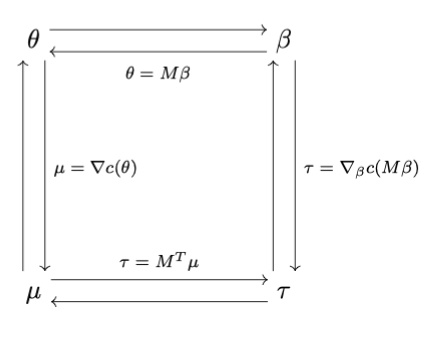
\includegraphics{transformations.png}
\end{frame}

\begin{frame}{}
\protect\hypertarget{section-3}{}
\textbf{Note}: \(\mu \to M^T\mu\) is usually not one-to-one (when
\(n > p\) and \(M\) is full column rank).

Hence we cannot determine \(\hat\theta\) and \(\hat\beta\) from them
either.

The only way to determine the MLEs is to maximize the log likelihood
\eqref{subloglike} to obtain \(\hat\beta\) and then

\begin{itemize}
\tightlist
\item
  \(\hat\theta = M\hat\beta\)
\item
  \(\hat\mu = \nabla c(\hat\theta)\)
\item
  \(\hat\tau = M^T\hat\mu\).
\end{itemize}
\end{frame}

\begin{frame}{GLMs and link functions}
\protect\hypertarget{glms-and-link-functions}{}
Recall that the saturated model canonical parameter vector \(\theta\) is
\emph{linked} to the saturated model mean value parameter vector through
the change-of-parameter mappings \(g(\theta)\).

\vspace{12pt}

We can reparameterize \(\theta = M\beta\) and write \[
 \mu = \text{E}_\theta(Y) = g(M\beta) 
\] which implies that we can write \[
  g^{-1}\left(\text{E}_\theta(Y)\right) = M\beta.
\]
\end{frame}

\begin{frame}{}
\protect\hypertarget{section-4}{}
Therefore, a linear function of the canonical submodel parameter vector
is linked to the mean of the exponential family through the inverse
change-of-parameter mapping \(g^{-1}\).

\vspace{12pt}

This is the basis of exponential family generalized linear models with
link function \(g^{-1}\).

\vspace{12pt}

Note that most treatments of GLMs will present \(g^{-1}\) as the link
function. Instead we motivated a change of parameters mapping from
canonical to mean value parameters.
\end{frame}

\begin{frame}{Example: logistic regression}
\protect\hypertarget{example-logistic-regression}{}
Logistic regression is a different form of regression with binary
outcomes.

\vspace{12pt}

Data is observed in independent pairs \((y_i,x_i')\),
\(i = 1\),\(\ldots\),\(n\) where the covariates are assumed to be known.

\vspace{12pt}

The idea is the probability of success changes with covariates in the
following manner \[
  p_i = P(Y_i|x_i) = f(x_i'\beta)
\] where \(f:\mathbb{R}\to (0,1)\) is continuous and monotone.

\vspace{12pt}

We will study linear regression using \(f = g\). Other choices of \(f\)
will be considered later.
\end{frame}

\begin{frame}{}
\protect\hypertarget{section-5}{}
Let \(M\) have rows \(x_i'\), \(i = 1\), \(\ldots\), \(n\).

Then \(\theta_i = x_i'\beta\), \[
  g(x_i'\beta) = \left(\frac{\exp(x_i'\beta)}{ 1 + \exp(x_i'\beta)}\right) = p_i,
\] and \[
  g^{-1}(p_i) = \log\left(\frac{p_i}{1 - p_i}\right) =  x_i'\beta. 
\]
\end{frame}

\begin{frame}{}
\protect\hypertarget{section-6}{}
We can write the log likelihood in canonical form in the saturated model
parameterization starting from the log likelihood of independent
Bernoulli trials: \begin{align*}
  &\sum_{i=1}^n\left[y_i\log(p_i) - (1 - y_i)\log(1 - p_i) \right] 
  %= \sum_{i=1}^n\left[y_ix_i'\beta - \log(1 + \exp(x_i'\beta))\right] \\
  %  &= \sum_{i=1}^n\left[\langle y_i, x_i'\beta \rangle - \log(1 + \exp(x_i'\beta)) \right] \\
  %  &= \langle y, \theta \rangle - \sum_{i=1}^n \log(1 + \exp(\theta_i)) \\
  = \langle y, \theta \rangle - c(\theta). 
\end{align*}
\end{frame}

\begin{frame}{}
\protect\hypertarget{section-7}{}
Alternatively, we can write the log likelihood in canonical form in the
submodel parameterization starting from the log likelihood of
independent Bernoulli trials: \begin{align*}
  &\sum_{i=1}^n\left[y_i\log(p_i) - (1 - y_i)\log(p_i) \right] 
  %&\sum_{i=1}^n\left[\langle y_i, x_i'\beta \rangle - \log(1 + \exp(x_i'\beta)) \right] \\
  %&= \langle \sum_{i=1}^n y_i x_i, \beta \rangle - \sum_{i=1}^n\log(1 + \exp(x_i'\beta)) \\
  = \langle M'y, \beta \rangle - c_\beta(\beta)
\end{align*}
\end{frame}

\begin{frame}{Difference in symmantics}
\protect\hypertarget{difference-in-symmantics}{}
\[
  \nabla_\beta c(\theta) = \nabla_\beta c(M\beta) = M^T\left[\nabla_\theta c(\theta)|_{\theta = M\beta}\right]
\] vs \begin{align*}
   \nabla_\beta c_\beta(\beta) = %\nabla_\beta \left[\sum_{i=1}^n\log(1 + \exp(x_i'\beta))\right] \\
     %&= \sum_{i=1}^n x_i \left[\frac{\exp(x_i'\beta)}{1 + \exp(x_i'\beta)}\right] \\ 
     %&= \sum_{i=1}^n x_i\left[\nabla_{\theta_i} c(\theta_i)|_{\theta_i = x_i'\beta}\right] \\ 
     %&= 
     M^T\left[\nabla_\theta c(\theta)|_{\theta = M\beta}\right].
\end{align*}
\end{frame}

\begin{frame}{Inference}
\protect\hypertarget{inference}{}
We have a regular full exponential family submodel with log likelihood
written in canonical form \[
    l(\beta) = \langle M^Ty,\beta \rangle - c(M\beta)
\]

From here, we have that the asymptotic distribution of the MLE
\(\hat\beta\) takes the form \[
  \sqrt{n}\left(\hat\beta - \beta\right) \overset{d}{\to} N(0, \Sigma^{-1})
\] where \(\Sigma = \text{E}\left(-\nabla_\beta^2 l(\beta)\right)\) is
the Fisher information matrix corresponding to the canonical linear
submodel.
\end{frame}

\begin{frame}{Wald inference for \(\beta\)}
\protect\hypertarget{wald-inference-for-beta}{}
Let \(\widehat\Sigma\) be estimated \(\Sigma\) using the MLE
\(\hat\beta\) in place of \(\beta\). In particular, the \(j\)th element
\(\hat\beta_j\) of \(\hat\beta\) is asymptotically normal with
asymptotic variance \[
  \widehat{\text{Var}}(\hat\beta_j) = jth \; \text{diagonal element of} \; \widehat\Sigma.
\]

\vspace*{12pt}

The Wald \(Z\) statistic for testing \(H_o:\beta_j = \beta_{jo}\) is \[
  z_W = \frac{\hat\beta_j - \beta_{jo}}{\text{se}(\hat\beta_j)} \quad \overset{H_o}{\sim} \quad N(0,1)
\] where se\((\hat\beta_j) = \sqrt{\widehat{\text{Var}}(\hat\beta_j)}\).
\end{frame}

\begin{frame}{}
\protect\hypertarget{section-8}{}
We can construct \((1-\alpha)\times 100\%\) Wald based confidence
intervals of the form \[
  \hat\beta_j \pm z_{\alpha/2}\text{se}(\hat\beta_j)
\] for some error tolerance \(0 < \alpha < 1\).
\end{frame}

\begin{frame}{Inference for mean value parameters}
\protect\hypertarget{inference-for-mean-value-parameters}{}
One could consider a function \(f:\beta\to\mu\) and then estimate the
variance of \(\hat{\mu}\) via the Delta method. One could then use Wald
inference.

\vspace{12pt}

Alternatively, we could use the change of parameters map and plug-in: \[
  \left[g(\hat\beta - z_{\alpha/2}\text{se}(\hat\beta), g(\hat\beta + z_{\alpha/2}\text{se}(\hat\beta) \right]
\]

\vspace{12pt}

\begin{itemize}
\tightlist
\item
  The former has the advantage that it is derived from principles.
\item
  The latter has the advantage that it will always return valid values
  for mean value parameters.
\end{itemize}
\end{frame}

\begin{frame}{Deviance, goodness of fit, and likelihood inference}
\protect\hypertarget{deviance-goodness-of-fit-and-likelihood-inference}{}
To motivate the deviance of a statistical model we will rewrite the log
likelihood as \(l(\mu;y)\).

The unrestricted MLE of \(\mu\) is \(y\). Now consider a canonical
submodel (GLM) of the form \(\theta = M\beta\).

Let \(\hat\mu\) be the MLE of \(\mu\) restricted to an identifiable
canonical submodel (\(\hat{\mu} = \nabla c(\hat\theta)\) where
\(\hat\theta = M\hat\beta\)). It follows that \[
  l(y;y) \geq l(\hat\mu; y).
\]

The \emph{deviance} of the GLM is \[
  D(y;\hat\mu) = -2\left(l(\hat\mu;y) - l(y;y)\right).
\]
\end{frame}

\begin{frame}{}
\protect\hypertarget{section-9}{}
The deviance statistic has approximate distribution \[
  D(y;\hat\mu) \; \overset{H_o}{\sim} \; \chi^2_{\text{df}}
\] where \(H_o\) is that the canonical submodel is correct and the
alternative test is that the canonical submodel is incorrect but the
saturated model is correct where

\begin{itemize}
\tightlist
\item
  df = \(n - p\)
\item
  \(n\) is the sample size
\item
  \(p\) is the number of parameters in the canonical submodel.
\end{itemize}
\end{frame}

\begin{frame}{}
\protect\hypertarget{section-10}{}
We reject correctness of the canonical submodel when \[
  D(y;\hat\mu) \; > \: \chi^2_{\text{df}}(\alpha).
\] (Note that the \(\chi^2\) approximation can be poor.)

\vspace{12pt}

Wait, isn't this backwards?
\end{frame}

\begin{frame}{A brief look at sufficiency}
\protect\hypertarget{a-brief-look-at-sufficiency}{}
\begin{lem}
The canonical statistic vector of an exponential family is a sufficient statistic.
\end{lem}

\vspace{12pt}

In other words, if \(\theta = M\beta\) yields \[
  D(y;\hat\mu) \; < \: \chi^2_{\text{df}}(\alpha),
\] then we have sufficient dimension reduction from \(n\) to \(p\).
\end{frame}

\begin{frame}{Deviance testing for nested submodels}
\protect\hypertarget{deviance-testing-for-nested-submodels}{}
Let \(\mathcal{M}_0\) and \(\mathcal{M}_1\) both be canonical submodels.

\vspace{12pt}

We say that \(\mathcal{M}_0\) is \emph{nested} within \(\mathcal{M}_1\)
when every distribution in \(\mathcal{M}_0\) is also in
\(\mathcal{M}_1\) but not vice-versa.

\vspace{12pt}

That is, \(\mu\) is more restricted under \(\mathcal{M}_0\) than under
\(\mathcal{M}_1\). Another way to look at it is that \[
  M_1 = \left[M_0, A \right],
\] where

\begin{itemize}
\tightlist
\item
  \(M_0\) is the model matrix for model \(\mathcal{M}_0\)
\item
  \(M_1\) is the model matrix for model \(\mathcal{M}_1\)
\item
  \(A\) represents additional covariates collected for all individuals
\end{itemize}
\end{frame}

\begin{frame}{}
\protect\hypertarget{section-11}{}
Let

\begin{itemize}
\tightlist
\item
  \(\hat\mu_0\) be the MLE of \(\mu\) under \(\mathcal{M}_0\)
\item
  \(\hat\mu_1\) be the MLE of \(\mu\) under \(\mathcal{M}_1\).
\end{itemize}

\vspace{12pt}

We can use this framework for testing \[
  H_0:\mathcal{M}_0 \; \text{true} \qquad H_a:\mathcal{M}_1 \; \text{true, but not} \; \mathcal{M}_0
\] using the likelihood ratio \(\chi^2\) statistic given by
\begin{align*}
 -2\left[l(\hat\mu_0;y) - l(\hat\mu_1;y)\right] %&= -2\left[l(\hat\mu_0;y) - l(y;y)\right] 
   %- \left\{-2\left[l(\hat\mu_1;y) - l(y;y)\right]\right\} \\
   %&= D(y;\hat\mu_0) - D(y;\hat\mu_1) \\ 
   &\approx \chi^2_{\text{df}}, 
\end{align*} where

\begin{itemize}
\tightlist
\item
  df = \(p_1 - p_0\)
\item
  \(p_1\) is the number of parameters in \(\mathcal{M}_1\)
\item
  \(p_0\) is the number of parameters in \(\mathcal{M}_0\).
\end{itemize}

(Note that the \(\chi^2\) approximation is often adequate here even it
isn't adequate for the saturated model provided that \(\mathcal{M}_1\)
is not too close to saturated.)
\end{frame}

\end{document}
